\documentclass[a4paper, 12pt, twoside]{article}
\usepackage{fancyhdr}
\usepackage{amsmath}
\usepackage{graphicx}

\pagestyle{fancy}
\fancyhf{}
\rhead{Joseph Free \\ MATH 3261 \\ Project 4}
\lhead{Solving a Linear System using the Gauss-Seidel Method}
\addtolength{\headheight}{41.7pt}
\cfoot{\thepage}

\begin{document}
\section{Problem}
In this assignment we will being utilizing the Gauss-Seidel method to approximate the solution of a linear system within $10^{-5}$
in the $l_\infty$ norm. The system in question is 

\begin{equation}
\label{one}
\begin{array}{rrrrr}
2x_1& -x_2& + x_3& = & -1\\
2x_1& +2x_2& + 2x_3& = & 4\\
-x_1& -x_2& + 2x_3& = & -5.\\ 
\end{array}
\end{equation}

To obtain the iterative method we intend to use, we isolate the diagonal and lower triangular terms on one side of the equality signs, which yields

$$
\begin{array}{ccccccc}
2x_1& & & = & -1 & +x_2& - x_3\\
2x_1& +2x_2& & = & 4 & - 2x_3\\
-x_1& -x_2& + 2x_3& = & -5.\\ 
\end{array}
$$

Converting the system into matrix form, we have

\begin{equation}
\label{two}
\begin{bmatrix}
2&	0&	0\\
2&	2&	0\\
-1& -1& 2\\
\end{bmatrix}
\begin{bmatrix}
x_1\\x_2\\x_3\\
\end{bmatrix}
=
\begin{bmatrix}
0&	1&	-1\\
0&	0&	-2\\
0&	0&	0\\
\end{bmatrix}
\begin{bmatrix}
x_1\\x_2\\x_3\\
\end{bmatrix}
+
\begin{bmatrix}
-1\\4\\-5\\
\end{bmatrix}
\end{equation}

Let the coefficient matrices on the L.H.S. and R.H.S. be denoted by $D+L$ and $U$, respectively, and let $C$ be the constant vector $(-1,4,-5)^t$. Furthermore, let the vector $(x_1, x_2, x_3)^t$ on the R.H.S. be the $kth$ term of the sequence $\left\lbrace \textbf{x}^{(n)} \right\rbrace$, and let the same vector on the L.H.S. be  the $(k-1)th$ term of the sequence. Then, we can express (\ref{two}) as

$$(D+L)\textbf{x}^{k} = U\textbf{x}^{k-1} +C.$$

Then, assuming that $D+L$ is non-singular, we can isolate $\textbf{x}^{k}$ and obtain

$$
\begin{array}{rrrrr}
\textbf{x}^{k}& = &(D+L)^{-1}U\textbf{x}^{k-1}& +&(D+L)^{-1}C\\
\\
&=&\begin{bmatrix}
0&1/2& -1/2\\
0&-1/2&-1/2\\
0&0&-1/2\\
\end{bmatrix}
\textbf{x}^{k-1}
&+&
\begin{bmatrix}
-1/2\\5/2\\-3/2\\
\end{bmatrix}
\end{array}
$$
which is exactly the Gauss-Seidel iterative method. 

The matrix $(D+L)^{-1}U$ is called the Gauss-Seidel matrix, and if its Spectral Radius lies within the unit disk ($\lvert z \rvert < 1$), the sequence $\left\lbrace \textbf{x}^{(n)} \right\rbrace$ is guaranteed to converge to the solution of (\ref{one}). For this particular problem, it is easily verifiable that $\lvert\rho((D+L)^{-1}U)\rvert = 1/2$, hence we may proceed without any problems.
\newpage

\section{Source Code}
$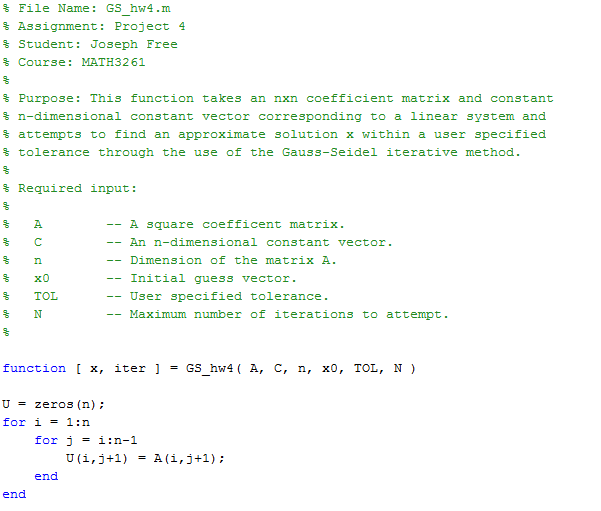
\includegraphics{GS_hw4_1}$
\newpage
$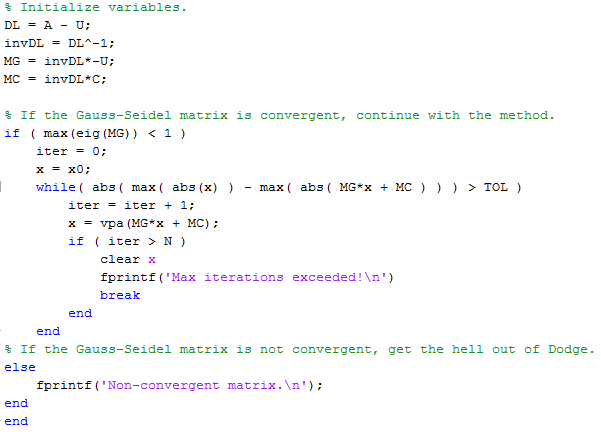
\includegraphics{GS_hw4_2}$
\newpage
$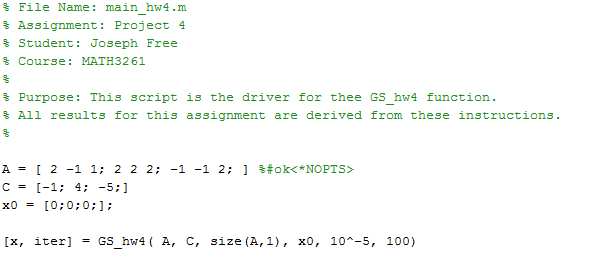
\includegraphics{main_hw4}$
\newpage

\section{Results}
As seen in the Source Code section above, in the main\_hw4 script we supply the function GS\_hw4 with the coefficient matrix and constant vector from (\ref{one}), the dimension of the matrix, an initial guess vector of $(0,0,0)^t$, tolerance of $10^-5$, and a maximum number of iterations. Using this data the GS\_hw4 function constructs the Gauss-Seidel matrix, checks the criterion for convergence, and then proceeds to iterate through the sequence. Upon completion, it will yield the approximate solution $\textbf{x}$ in addition to the number of iterations required to reach within $10^-5$ of the actual solution. The results proper can be seen below:
\begin{center}
$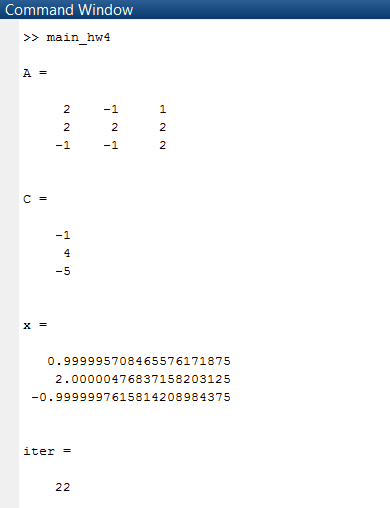
\includegraphics{output_hw4}\centering$
\end{center}

Thus, we see that after 22 iterations, we have a sufficiently accurate approximation to the solution of (\ref{one}).
\end{document}
